\chapter{Further Work} \label{chapter:further}
The whole project was intended to be a prototype to see if feature classification could be implemented using OS images, hence this covered basic functionality. Allowing many ways to improve the current system. In some sections there are mentions of further work that are specific to a particular module. Due to the modularity associated with Microservices and the structure of our code, a solid foundation is set to enable extensions and improvements. This chapter includes some of these potential system improvements and extensions




\section{Improvements}


\subsection{Example training usage}
One outcome from the usability testing at OS was that users were not entirely sure how to classify various tiles. Given that tiles covered more than one specific type of feature e.g. a tile containing a house that backed onto a forest; they were unsure how to handle mixed theme tiles.

They suggested that a demonstration to be included on the web-site. This could be simply a collection of images and what classifications they should be deemed as. This would provide a guide and more confidence to the users when the Productizer is in learn mode. This could be included in the learn mode, scrolling down to see it. 




\subsection{Required Training Indicator}
One issue we observed through the usability testing was that the users assumed the system was ready to `discover' features far earlier than it would be recommended to. This resulted in bad or obviously untrustworthy classifications from the `discover sweep'. To account for this there should be stricter control over when user trains classifier on any given theme. This can be achieved by implementing some kind of GUI based indicator bar within the site that will hint the user on how many more tiles for each feature type are required to ensure a respectable and reliable outcome. 


\subsection{Normal Curve Context}
The current implementation extracts `context' from inside the tile and only the tile. As a result there is an issue when classifying regions that are bigger than a tile. For example the difference between a pond and lake or a larger private garden or public park. Features are normally very related to their surroundings. The NSEW approach ignores  surrounding tiles.

A way to solve this would be by extending the context to a larger number of tiles. The solution would involve two stages of classification in order to determine the final classification: 
\begin{enumerate}
\item Classification of all the NSEW generated sub-tiles
\item A weighted sum of classifications where the weighting is determined by a bell curve

\end{enumerate}

The first classification is the same as the current format however the resulting label of each sub-tile would be stored in graph of nodes. This would created a 2D network, where every node has an x and y position and a class label. 


The second classification would look at each tile $t$ and weigh each surrounding node based on its position on the bell curve. The bell curve would have a mean $ \mu $ (or centre) of the centre of the tile $\mu = \begin{bmatrix}x_t \\ y_t \end{bmatrix}.$

\begin{figure}[H]
    \centering
    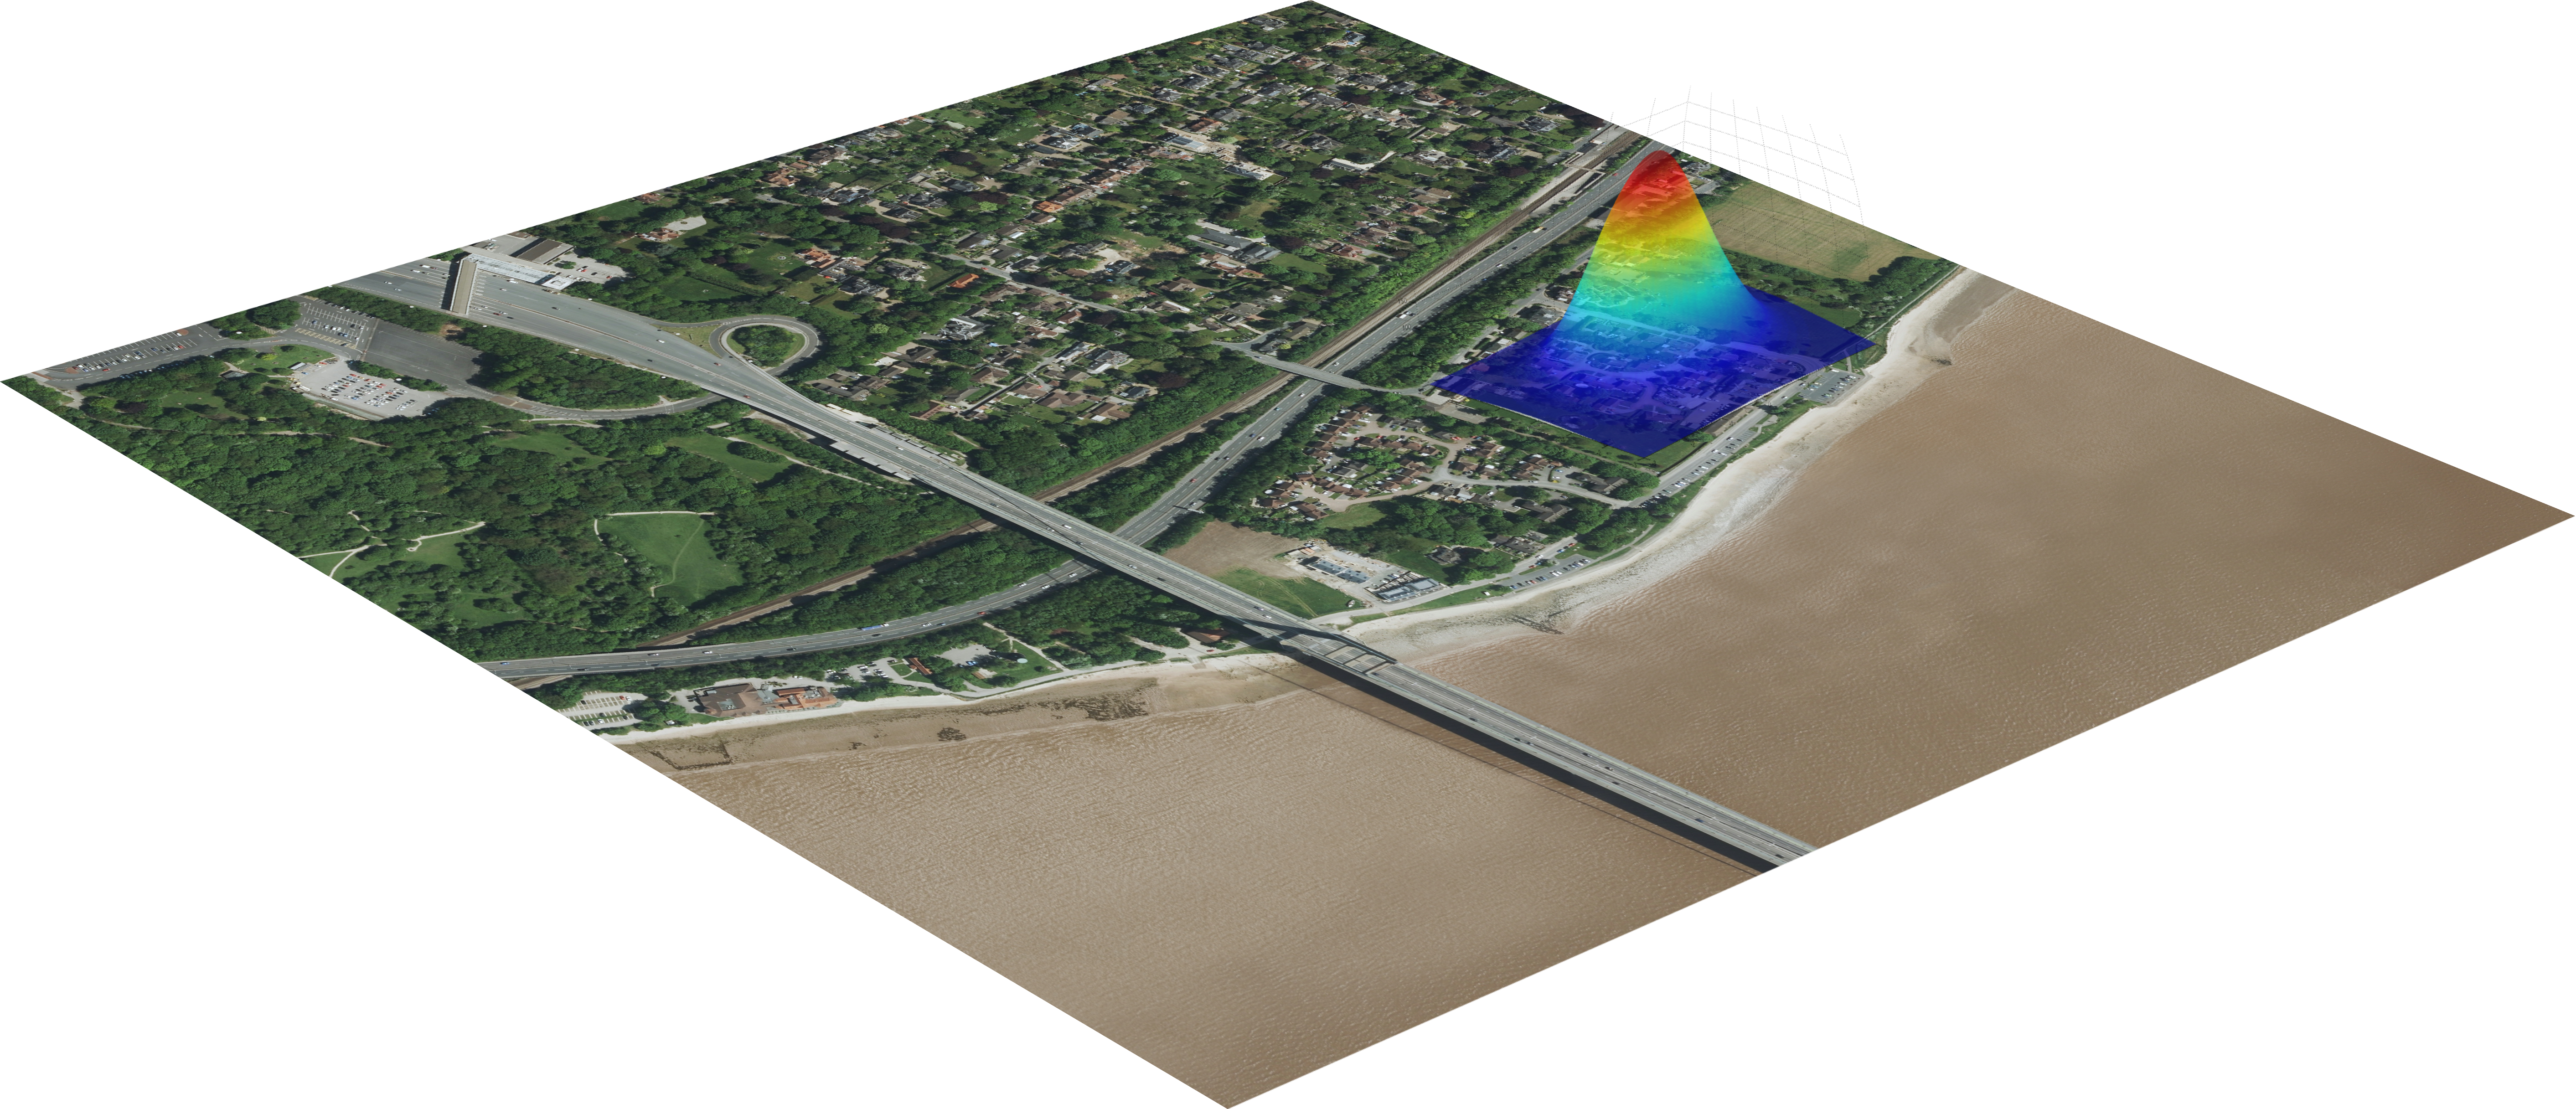
\includegraphics[width=\textwidth]{figs/12/3d_normal}
    \caption{A 3D representation of the normal curve}
    \label{fig:fw:3d_normal}
\end{figure}

Previously a tile would contain 9 nodes (each NSEW result) and each classified node would carry a weight of $11.1\%$. 
In the proposed method, nodes outside the tile will have an influence on the final classification. 
Figure \ref{fig:fw:3d_normal} shows that weight. 
The distance of a node $n = \begin{bmatrix}x_n \\ y_n \end{bmatrix}$
from the centre of the tile provides an weight of $P(T = n)$ 
such that $T \sim \mathcal{N}(\mu,\,C)\,$, 
where the co-variance $C  =\begin{bmatrix}\sigma^2 & 1 \\ 1 & \sigma^2 \end{bmatrix}$.\\
Minor normalisation might have to occur, in order to prevent a total of 100\%. 
Therefore probability for a tile $t$ belonging to any class $f$:

$$ 
P(f | t)  =
\Phi \Bigg(
\sum_{i=(x_t-2\sigma)}^{(x_t+2\sigma)}
\sum_{j=(y_t-2\sigma)}^{(y_t+2\sigma)}
\Big(
\lambda_{i,j}(f) \cdot P(T = t)
\Big)
\Bigg)
$$

Such that $\Phi(x)$ is the normalisation function and the binary function $\lambda_{i,j}(f)$ equals 1 if the node at [i,j] was initially classified as feature $f$ and 0 otherwise.


$$
\lambda_{i,j}(f) = 
\begin{cases}
\mbox{1} & \text{if SVM.classify}(n) = f\\
\mbox{0} & \text{otherwise}
\end{cases}
$$

The winning feature $\hat{f}$ for the tile would be the feature with the highest probability:
$P(\hat{f}|t) > P(f|t)\ \forall f \neq \hat{f}$. 






\subsection{Required Training Indicator}
Given an incorrect classification, currently a user must switch from discover to learn mode; then find the incorrectly labelled tile and correctly retrain the model with that feature. This raises two issues. Switching from discover to learn mode removes all the markers. Which firstly, makes it difficult to find the exact tile. Secondly you cannot see what it was classified as. 

To solve this, there should be some sort of button allowing the user to make an amendment on the discover mode. Based on the design of the system, it would be (computationally) optimal for the user to queue a number of corrections. As batches of information take less time to process. However this may be less intuitive. To counter this, the queue should be hidden from the user. The classification will enter a pending state, where it will await for the user to change mode or click the reclassify button. Changing mode would send all amendments to Saturn as if it was a standard learn mode with mixed label data. If the user clicked `reclassify' originally, a discover sweep would occur. However in this case a hidden (i.e. the user will not be informed) learn command (without changing to learn mode) would be sent, followed by a `discover' sweep, so that the changes affect the reclassification.  





\section{Extensions}
\subsection{Automation of learning via MasterMap}
OS has a number of map products containing all sorts of information. Their flagship product is `OS MasterMap'. It contains over 470 million features and is constantly being updated (10,000 features a day, \cite{OS:Youtube}). The classifications of these features is expansive, such as marshes, post offices, pylons, telephone boxes and more. This expansive amount of labelled data could be used to replace the human operator during training. MasterMap also has a aerial imagery layer. As the two products are MasterMap, their coordinate system would match, therefore creating corresponding tiles would be trivial. By automating the process of learning the data, an operator needs only to correct mistakes. Which would mainly be edges cases.

Once a selection of tiles has been generated, the issue of classifying a tile arises. This could  be solved in two ways. The first way could be by determining how much of the tile is covered by each feature within a tile area and the tile is classified as the feature with the largest area. The second method would mimic the NSEW approach. Where nine points are taken from the tile in the same location as the nine focus points of the NSEW approach. The feature type at that exact location would be a vote for that feature type. The feature type with the most vote claims the tile.

\begin{figure}[H]
    \begin{minipage}{0.5\textwidth}
  \centering
  \includegraphics[width=0.95\textwidth]{figs/12/osmm_m1}
  \caption{Method 1}
  \label{fig:sub2}
\end{minipage}\hfill
\begin{minipage}{0.5\textwidth}
  \centering
  \includegraphics[width=0.95\textwidth]{figs/12/osmm_m2}
  \caption{Method 2}
  \label{fig:sub2}
\end{minipage}
\caption{Two methods of choose a class for a tile}
\label{fig:FW:methods}

\end{figure}



If we compare the two methods in the example in Figure \ref{fig:FW:methods}, the second method seems more optimal. Housing wins with a vote of 5 to 4 for gardens, whereas the first method would result in garden as it obviously has the largest area (yellow). However this would need to be experimented as this is a single case; a potentially more complex method might need to be adopted. 

No internal code changes are required, due to the nature of the micro-services. However, a new simple controller would be needed, to orchestrate the task. Assuming the tagging of tiles before training the model can be achieved, this allows for more training data to be processed in less time. The more a model is trained, the more reliably it can classify the correct feature to a tile. This allows the model to rapidly update when a new collection of data arrives. By training it on random tiles it can quickly learn the entire new dataset and propagate the knowledge classifying all of it.







\subsection{Discover Feature Outlines}
A common theme that resonates throughout the system is the issue with tiles. Raw tiling is a flawed system for identifying specific features. Within a single tile there could be multiple features that we have to generalise to a single feature; resulting in an effective loss of data. 

If we could extract objects from a tile, we could then attempt to classify the single objects. This can be done by in a number of ways. A simple yet effective method would be edge detection, the most appropriate method from similar works seems to be the Sobel method with a binary gradient mask in order to determine object outlines \citep{sobel_method}. The outlines can then be applied to cut the objects from the tile. 

\begin{figure}[H]
    \centering
    \includegraphics[width=\textwidth]{figs/12/sobel}
    \caption{Potential results of object extraction}
    \label{fig:FW:sobel}
\end{figure}

Figure \ref{fig:FW:sobel} shows an example of what you would hope the edge detection would produce. Note that a light green colour was taken to show that the remaining image has been ignored. With these new images each region \textbf{within} a tile can be classified, also leaving unknown or miscellaneous regions that request human assistance. More importantly this would produce a more precisely classified map. As can be shown in the figure \ref{fig:FW:object_class}, the results are quite dramatically different. 

\begin{figure}[H]
    \centering
    \includegraphics[width=\textwidth]{figs/12/new_classes}
    \caption{Comparison of Object classification verses tiling classification}
    \label{fig:FW:object_class}
\end{figure}